\providecommand{\main}{..}
\documentclass[\main/main.tex]{subfiles}

\begin{document}
\lesson{15}{18/11/20}

\subsection{Mean-field theory}
In analogy with equilibrium phase transitions, it has been conjectured that the notion of universality applies also to continuous non-equilibrium phase transitions. This means that scaling properties characterizing the behavior close to the critical point depend on basic properties only and are independent of the details of the model at hand. It is worth pointing out that such a conjecture has been successfully checked in many cases by
careful numerical studies, but a rigorous mathematical proof is still unknown, because the dynamical renormalization group method encounters more serious technical difficulties to be worked out than the static one. \\

What we will do is writing a phenomenological Langevin equation for a quantity called $\rho(\Vec{x},t)$ which is the density of active sites at position $\Vec{x}$ and at time $t$.
This quantity has to be understood as a space-time coarse-grained average. \\

Let's start with a further approximation in which we consider a uniform density \marginpar{Mean-field treatement of contact processes}of active sites $\rho(\Vec{x},t)$ with a \textit{contact process}, which is actually a very simple example to model epidemic spreading. The fact of talking about contact processes is to emphasize the concept of 'universality': the detail of the model that we will preset will be different from DP but it belongs to the same class of universality. \\

Let's call active sites \textit{infected individuals} and empty becomes \textit{healthy individuals}: if all individuals stay healthy (empty) then the others will be healthy too but if we have a single initially infected individual (\textit{patient zero}).

\begin{figure}[ht]
    \centering
    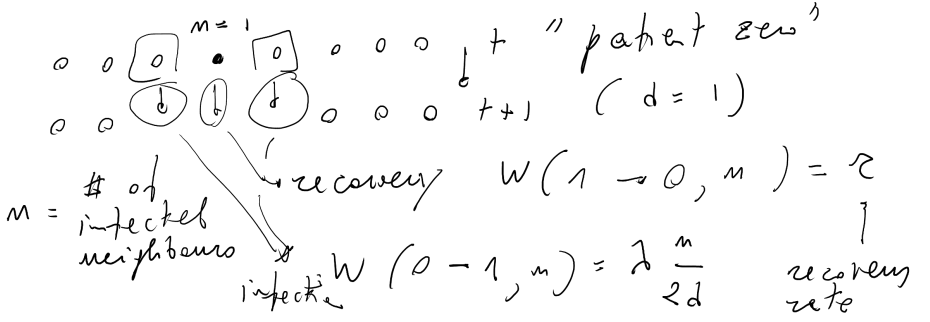
\includegraphics[width=\linewidth]{Lectures/Images/qi.png}
    \caption{Contact process: epidemic spreading example, where 0 corresponds to empty/healthy while 1 corresponds to active/infected.}
    \label{fig:pandemic}
\end{figure}

A first difference with DP can be seen in Figure \ref{fig:pandemic}: in this example we are not using a tilted lattice and we can recognize two different processes going on, \textit{infection} and \textit{recovery}.

People who were infected can recover and the probability that describes this event is defined as the \textit{recovery rate} $r:=w(1\to 0,n)$. In principle this rate\footnote{Not so precise: we are describing a discrete time model defining rates as if the time was continuous.} could depend on $n$ i.e. on the number of infected neighbours: for example in Figure \ref{fig:pandemic} for the squared sites $n$ corresponds to one because they both have an infected neighbour.

In the simplest case recovery does not depend on the number of infected neighbours and is a given probability $r$.

For what concerns infection we can decide whether an infected site stay infected or get healthy just depending on the recovery rate but we also must have a rule for infection: one possible rule is $w(0\to 1,n)=\lambda n/2d$, where $\lambda$ is the \textit{infection rate} i.e. the probability of being infected by a neighbour in one timestep and in the sketch (which is in $d=1$ but we are formulating it in $d$ dimensions) $n/2d$ is the fraction of infected neighbours (because $2d$ is the number of nearest neighbours). \\

This model belongs to the \textbf{same universality class of DP} and numerically\footnote{No analytic solutions even for $d=1$.} we can show that the critical ratio of the transition threshold $(\lambda/r)_c\simeq 3.29785$.

In this very simple model \textit{reinfection} is allowed: one a given individual is recovered it can be infected again. \\

Let's now introduce the mean-field approach\marginpar{Mean-field} with uniform density of infected sites $\rho(t)$. The mean-field evolution equation, switching to continuous time, is:
\begin{equation}
    \frac{\partial \rho}{\partial t}=\underbrace{\lambda \rho(\hlc{yellow}{1-\rho})}_{\text{gain term}}-\underbrace{r\,\cdot \hlc{green}{\rho}}_{\text{loss term}} := a \rho-\lambda \rho^{2}
\end{equation}
where the yellow term is the healthy one, while the green term is the infected one and the linear term is defined as $a:=\lambda - r$; this is a mean-field approach because we are losing the fact that we have neighbours and everything is uniform.

Factorizing $\rho$ and looking for stationary solutions $\rho^*$:

\begin{equation}
    \frac{\partial \rho}{\partial t}=\rho(a-\lambda \rho) \quad s.t. \quad \frac{\partial \rho}{\partial t}\rvert_{\rho=\rho^*}=0
\end{equation}
then
\begin{numcases}{\partial_t \rho \rvert_{\rho^*}=0\,\, \iff \,\,}
    \rho_1^*=0 \\
    \rho_2^*=\frac{a}{\lambda}=\frac{\lambda-r}{\lambda}=1-\frac{r}{\lambda}
\end{numcases}

when are $\rho_{1,2}^*$ stable or unstable? Let's compute the second derivative:
\begin{equation}
    \derparstwo{t}\rho=a-2\lambda\rho\quad\implies \quad \derparstwo{t}\rho\rvert_{\rho=\rho_1^*}= a; \,\,\, \derparstwo{t}\rho\rvert_{\rho=\rho_2^*}= -a;
\end{equation}
and so
\begin{numcases}{\text{if}\,\,\,}
    a>0 \longrightarrow \rho_2^* & is stable and $\rho_1^*$ is unstable; \\
    a<0 \longrightarrow \rho_2^* & is unstable and $\rho_1^*$ is stable; 
\end{numcases}
the solution $\rho_1^*=0$ is the inactive phase (all sites healthy), $\rho_2^*=a/\lambda$ is the active phase (epidemic spreading) and so even if we go to the thermodynamic limit a finite fraction of all sites are infected. 

To conclude we've found that the critical point  -in the uniform approach - is given by $a_c=0$ i.e. $(\lambda/r)_c=1$ (which is clearly different from 3.298): the mean-field approach under estimates the exact value of the critical threshold.n\\

Let's now consider a non-uniform density $\rho(\Vec{x},t)$ of active sites\marginpar{Non-uniform density of active sites}: mean-field means that stochastic fluctuations are neglected.

The overall aim is to get a mean-field calculation of a critical exponent: essentially we will write a Langevin-like equation for $\rho$, adding a diffusion term due to the fact that $\rho$ isn't uniform anymore and a stochastic noise $\eta$

\begin{equation}
    \frac{\partial \rho(\vec{x}, t)}{\partial t}=a \rho(\vec{x}, t)-\lambda \rho^{2}(\vec{x}, t)+D \nabla^{2} \rho(\vec{x}, t)+\eta(\vec{x}, t)
    \label{eq:langevin_stoch}
\end{equation}

we will define the noise in a different way with respect to the Langevin equations used so far for the presence of the blue term (but it's still uncorrelated in space and time):
\begin{align}
    \mean{\eta({\vec{x}},t)}=0;\quad \quad \mean{\eta(\vec{x},t)\eta(\vec{x}',t')}=\Gamma \hlc{blue}{\rho(\vec{x},t)}\delta(\vec{x}-\vec{x}')\delta(t-t')
\end{align}

This is an example of \textit{multiplicative noise}\marginpar{Multiplicative noise} and we need to consider noise in such a way because noise is present only in the active phase.
In the active phase, in which all sites are healthy/empty, there is no fluctuation/ noise and $\rho=0$ everywhere.

Looking at physical dimensions we can realize that the strength $\Gamma = [s^{-1}]$.

In general the noise correlation tells us that 
\begin{align}
    \eta(\vec{x},t)\sim \sqrt{\rho(\vec{x},t)}
\end{align}

Let's now deduce the values of the critical exponents in the mean-field approach: the trick is to use \textit{scaling invariance} close to the critical point $a_c=0$ (we already found it in the context of uniform density).

In the last lecture we saw an example of scaling transformation with scaling factor $\Lambda$ that we chose to be equal to the distance from the critical point, which can say it's equal to $a$ because the critical point is $a=0$:
\begin{align}
    \Lambda=\Delta=a
\end{align}
Now we will write a rescaled Langevin equation applying (\ref{eq:scaling2}) to (\ref{eq:langevin_stoch}) taking into account that the distance $\Delta$ from the critical point is now equal to $a=\lambda-r$ because the critical point is defined precisely by the condition $a=0 .$ With the condition $\Lambda=a$ in mind (the yellow $(\beta)+1$ is due to this fact), the rescaled equation is
\begin{align}
\Lambda^{\beta+\nu_{\|}} \frac{\partial \rho(\mathbf{x}, t)}{\partial t} &=\Lambda^{\hlc{yellow}{\beta+1}} \rho(\mathbf{x}, t)-\lambda \Lambda^{2 \beta} \rho^{2}(\mathbf{x}, t)+ \\
&+ D \Lambda^{\beta+2 \nu_{\perp}} \nabla^{2} \rho(\mathbf{x}, t)+\Lambda^{\gamma} \eta(\mathbf{x}, t)
\label{eq:sc}
\end{align}
where the exponent\footnote{Riguarda 11.33 pt 2, non ho ben capito il perchè.} $\gamma=\left(\beta+d \nu_{\perp}+\nu_{\|}\right) / 2$ while taking into account the property of the Dirac delta distribution $\delta(c x)=\frac{1}{|c|} \delta(x)$.


Dividing all terms by $\Lambda^{\beta+\nu_{\|}}$ we obtain
\begin{align}
\frac{\partial \rho(\mathbf{x}, t)}{\partial t}&=\Lambda^{1-\nu_{\|}} \rho(\mathbf{x}, t)-\lambda \Lambda^{\beta-\nu_{\|}} \rho^{2}(\mathbf{x}, t)+\\
&+D \Lambda^{2 \nu_{\perp}-\nu_{\|}} \nabla^{2} \rho(\mathbf{x}, t)+\Lambda^{\hlc{yellow}{\gamma-\beta-\nu_{\|}}} \eta(\mathbf{x}, t)    
\label{eq:scasca}
\end{align}

If we impose that the deterministic part of the Langevin equation is invariant under scale transformations, we must impose the vanishing of the relative scaling exponents, which allows us to obtain
$$
\beta=\nu_\|=1, \quad \nu_{\perp}=\frac{1}{2}, \quad \nu_{\|}=1 \implies z=\frac{\nu_\|}{\nu_\perp}=2
$$

So far we've asked that the deterministic terms in the Langevin equation stay the same and we didn't consider yet the stochastic term: let's look at the stochastic term to determine the upper critical dimension.

\begin{appr}
When dealing with mean-field a limit in which we are sure mean-field treatment becomes exact is the limit of infinite dimension: in general what happens for any system is that there is an \textit{upper critical dimension} such that above that dimension the mean-field treatment provides exact results, so the exact results are the same of mean-field.
\end{appr}

The point is that mean-field exponents are exact when the stochastic term is \textbf{irrelevant} i.e. disappears in our scaling transformation (which implies that the yellow term of (\ref{eq:scasca}) must be positive because getting closer to the critical point means that $\Lambda$ is small) if $\gamma - \beta -\nu_\|>0$:
\begin{equation}
    \Lambda^{{\gamma-\beta-\nu_{\|}}}  \overset{\Lambda\to 0}{\longrightarrow} 0
\end{equation}

Substituting the value of $\gamma$ found in (\ref{eq:sc}) in the previous expression  we can find a condition on the dimension $d$:
\begin{equation}
    d\nu_\perp - \beta \nu_\|>0 \implies \boxed{d>\frac{\beta+\nu_\|}{\nu_\perp}=4}
\end{equation}
and in this way we were able to find the upper critical dimension, namely $d_c=4$, as in the Ising model, for instance.

This idea to check when mean-fields are exact by looking at the relevance of the\marginpar{Ginzburg criterion} stochastic term is known as \textit{Ginzburg criterion}. In mean-field we can also show that $\beta=\beta'$. \\

Recovering the scaling law for the $\theta$ exponent (which we didn't prove because it's difficult in the out-of-equilibrium phase transitions context)
\begin{equation}
    \theta=\frac{d\nu_\perp-2\beta}{\nu_\|} \overset{d=4}{=} 0
\end{equation}
this relation holds only for $d\leq 4$ and inn the context of mean-field: when we are at the upper critical dimension $d_c=4$ the mean-field exponents are also correct but with logarithmic corrections to the power law, therefore we  can use the scaling law for $\theta$ only with $d=4$ and if we do it we get as result zero.

\subsection{Different universality class (from DP)}
We again talking about non-equilibrium phase transitions and in particular the ones with absorbing states. We will show different examples on models where we move away from DP universality class.

An overall aim of this section will be to emphasize the similarity and the differences with respect to the case of equilibrium phase transitions.
In general, if we have in the model more absorbing phases, then we have a different universality class.

A way to change universality class can be expressed through a contact process example i.e. epidemic spreading: the reason why the following model belongs to another universality class is because it has more absorbing phases.

In DP we have only 1 absorbing phase: all sites are empty and the same was holding in the example of contact process with reinfection: all the individuals are healthy (unique absorbing state in the system if reinfection with the same probability $p_2 = \lambda n /(2d)$ is possible\footnote{Infection probability will be called $p_1$.}). \\

Let's complicate the model introducing the \textit{immunization}, which means that the idea that the reinfection probability $p_2$ is less than $p_1$.
We can talk about \textit{partial immunization} if still $p_2>0$.


We can have a complete immunization if we say that $p_2=0$ and this implies the use of a model called SIR, i.e. a given individual can be in 3 different states:
\begin{itemize}
    \item \textbf{S}usceptible (somebody who is originally healthy but never got the decease)
    \item \textbf{I}nfected 
    \item \textbf{R}ecover
\end{itemize}
Once the individual recovers can't be infected again because $p_2=0$.

In the perspective of non-equilibrium phase transitions with absorbing phases we can have more absorbing phases; in the previous example we have a n infinite number of possible absorbing phases/states. Any combination of S,R individuals will just say the same: the crucial thing to have an absorbing state is not have any infected individuals. \\

This is a way to change universality class: if $p_2=0$ and for small enough $p_2>0$ we can simulate the system at the critical point (based on the ratio of infection/recovery rate) finding that the critical exponent value are different from the DP case. \\

This universality class is called \textit{dynamical percolation}.

If $p_2=0$ the only parameter is $p_1$ and when $p_1>p_{1,c}$ where $p_{1,c}$ is a threshold value, we are in the active phase in which we have the propagation of a percolation front and not clusters anymore, while in the other case we are in the inactive phase

\section{SIR model}
It is a sort of mean-field approach with uniform $\rho$ (no spatial structure, time is the only parameters).

$N$ is the total number of individuals which is constant.
The partition of our system is based on 3 classes:
\begin{align}
    S(t)+I(t)+R(t)=N
\end{align}
and we have to deal with two parameters: $\lambda$ and $r$.
\begin{align}
    \lambda&=\frac{\textit{\#infected people by one infected individual}}{\textit{unit time}} \Longleftrightarrow \text{transition} S\to I \\
    r&=\frac{\textit{recover probability}}{unit time}=\frac{1}{t_r} \Longleftrightarrow \text{transition} I\to R 
\end{align}
where $t_r$ is the typical recovery time. \\
The equation for the SIR model is:
\begin{align}
    \frac{dS}{dt} &=-\lambda\frac{S}{N}I \\
    \frac{dI}{dt} &=\lambda\frac{S}{N}I-r I \\
    \frac{dR}{dt}&=rI
\end{align}
At epidemic start $S(t)\overset{<}{\sim}N$ and $I<<N$ and so we can approximate that $S/N=1$ and so the time evolution equation for the infected individuals becomes a close equation
\begin{align}
    \frac{dI}{dt}=(\lambda-r)I
\end{align}
whose solution is
\begin{align}
    I(t)=\exp{(\lambda-r)t}=\exp(r(\lambda/r-1)t)
\end{align}
where $R_0:=\lambda/r$ and it is called \textit{reproduction number} and it is the number of people infected by an individual before recovery. If $R_0=1$ critical threshold: $R_0>1$ active phase with exponential increase, $R_0<1$ exponential decrease.


\end{document}